%%%%%%%%%%%%%%%%%%%%%%%%%%%%%%%%%%%%%%%%%
% Beamer Presentation
% LaTeX Template
% Version 1.0 (10/11/12)
%
% This template has been downloaded from:
% http://www.LaTeXTemplates.com
%
% License:
% CC BY-NC-SA 3.0 (http://creativecommons.org/licenses/by-nc-sa/3.0/)
%
%%%%%%%%%%%%%%%%%%%%%%%%%%%%%%%%%%%%%%%%%

%----------------------------------------------------------------------------------------
%	PACKAGES AND THEMES
%----------------------------------------------------------------------------------------

\documentclass{beamer}

\mode<presentation> {

% The Beamer class comes with a number of default slide themes
% which change the colors and layouts of slides. Below this is a list
% of all the themes, uncomment each in turn to see what they look like.

%\usetheme{default}
%\usetheme{AnnArbor}
%\usetheme{Antibes}
%\usetheme{Bergen}
%\usetheme{Berkeley}
%\usetheme{Berlin}
%\usetheme{Boadilla}
\usetheme{CambridgeUS}
%\usetheme{Copenhagen}
%\usetheme{Darmstadt}
%\usetheme{Dresden}
%\usetheme{Frankfurt}
%\usetheme{Goettingen}
%\usetheme{Hannover}
%\usetheme{Ilmenau}
%\usetheme{JuanLesPins}
%\usetheme{Luebeck}
%\usetheme{Madrid}
%\usetheme{Malmoe}
%\usetheme{Marburg}
%\usetheme{Montpellier}
%\usetheme{PaloAlto}
%\usetheme{Pittsburgh}
%\usetheme{Rochester}
%\usetheme{Singapore}
%\usetheme{Szeged}
%\usetheme{Warsaw}

% As well as themes, the Beamer class has a number of color themes
% for any slide theme. Uncomment each of these in turn to see how it
% changes the colors of your current slide theme.

%\usecolortheme{albatross}
%\usecolortheme{beaver}
%\usecolortheme{beetle}
%\usecolortheme{crane}
%\usecolortheme{dolphin}
%\usecolortheme{dove}
%\usecolortheme{fly}
%\usecolortheme{lily}
%\usecolortheme{orchid}
%\usecolortheme{rose}
%\usecolortheme{seagull}
%\usecolortheme{seahorse}
%\usecolortheme{whale}
%\usecolortheme{wolverine}

%\setbeamertemplate{footline} % To remove the footer line in all slides uncomment this line
%\setbeamertemplate{footline}[page number] % To replace the footer line in all slides with a simple slide count uncomment this line

%\setbeamertemplate{navigation symbols}{} % To remove the navigation symbols from the bottom of all slides uncomment this line
}

\usepackage{graphicx} % Allows including images
\usepackage{booktabs} % Allows the use of \toprule, \midrule and \bottomrule in tables
\usepackage{multirow}
\usepackage{color}
\newcommand{\blue}[1]{\textcolor{blue}{#1}}
\newcommand{\red}[1]{\textcolor{red}{#1}}
\newcommand{\green}[1]{\textcolor{green}{#1}}
\newcommand{\yellow}[1]{\textcolor{yellow}{#1}}
\newcommand{\orange}[1]{\textcolor{orange}{#1}}
%----------------------------------------------------------------------------------------
%	TITLE PAGE
%----------------------------------------------------------------------------------------

\title[Circuit(ENGG 1203)]{Tutorial on Circuit (Part 1) \newline Introduction to Electrical and Electronic Engineering} % The short title appears at the bottom of every slide, the full title is only on the title page

\author{Nan Meng} % Your name
\institute[Imaging Systems Laboratory] % Your institution as it will appear on the bottom of every slide, may be shorthand to save space
{
	University of Hong Kong \\ % Your institution for the title page
	\medskip
	\textit{u3003637@connect.hku.hk} % Your email address
}
\date{\today} % Date, can be changed to a custom date

\begin{document}

\begin{frame}
	\titlepage % Print the title page as the first slide
\end{frame}

\begin{frame}
\frametitle{Overview} % Table of contents slide, comment this block out to remove it

\begin{itemize} \itemsep1pt \parskip0pt \parsep0pt
  \item[$\ast$] {\bf Learning Objectives:}\newline Analysis circuits through circuit laws (Ohm`s Law, KCL and KVL)
  \item[$\ast$] {\bf Basics}
  \begin{itemize} \itemsep1pt \parskip0pt \parsep0pt
    \item[$\bullet$] Symbols \& Rules
    \item[$\bullet$] Kirchhoffs Laws
    \begin{itemize} \itemsep1pt \parskip0pt \parsep0pt
      \item[$\bullet$] \red{Kirchhoffs Current Law(KCL)}
      \item[$\bullet$] \red{Kirchhoffs Voltage Law(KVL)}
    \end{itemize}
  \end{itemize}
  \item[$\ast$] {\bf Questions \& Summary}
\end{itemize}
\end{frame}

%----------------------------------------------------------------------------------------
%	PRESENTATION SLIDES
%----------------------------------------------------------------------------------------

%------------------------------------------------

%------------------------------------------------

\begin{frame}
\frametitle{Symbols \& Rules (Recap)}

\begin{itemize}
\item {\bf \blue{Voltage Source}}
\begin{columns}
\begin{column}{3cm}
\begin{figure}[H]
  \centering
  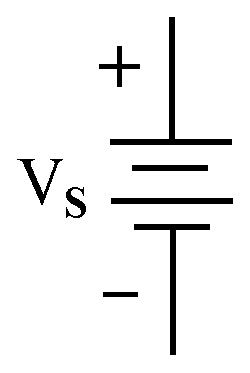
\includegraphics[width=0.4\textwidth,height=0.6\textwidth]{./image/circuit1/voltage1}
\end{figure}
\end{column}
\begin{column}{3cm}
\begin{figure}[H]
  \centering
  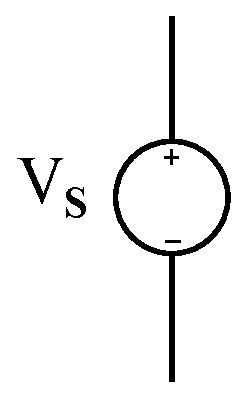
\includegraphics[width=0.4\textwidth,height=0.6\textwidth]{./image/circuit1/voltage2}
\end{figure}
\end{column}
\begin{column}{3cm}
\bf{\orange{Ideal (Direct) Voltage Source}}
\end{column}
\end{columns}
\item {\bf \blue{Current Source}}
\begin{columns}
\begin{column}{6cm}
\begin{figure}[H]
  \centering
  \includegraphics[width=0.18\textwidth,height=0.3\textwidth]{./image/circuit1/current1}
\end{figure}
\end{column}
\begin{column}{3cm}
~~\bf{\orange{Ideal (Direct) Current Source}}
\end{column}
\end{columns}
\item {\bf \blue{Resistor}}
\begin{columns}
\begin{column}{6cm}
\begin{figure}[H]
  \centering
  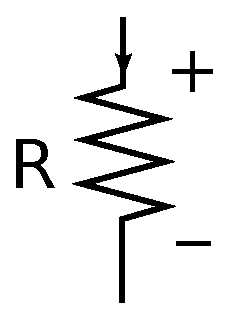
\includegraphics[width=0.18\textwidth,height=0.3\textwidth]{./image/circuit1/resistor}
\end{figure}
\end{column}
\begin{column}{3cm}
~~\bf{\orange{Resistor}}
\end{column}
\end{columns}
\end{itemize}

\end{frame}

%------------------------------------------------
\begin{frame}
\frametitle{Kirchhoff’s Laws (Recap)}

\begin{itemize}
\item {\bf \blue{Kirchhoff’s Current Law(KCL):}}
The current flowing out of any node in a circuit must be equal to the current flowing into the node.
\begin{equation}
\sum_{n=1}^{N}i_n=0
\end{equation}
where N is the number of branches that are connected to the node.


\item {\bf \blue{Kirchhoff’s Voltage Law(KVL):}}
The algebraic sum of voltages around a closed loop is zero.
\begin{equation}
\sum_{n=1}^{N}v_n=0
\end{equation}
where N is the number of voltages in the loop.
\end{itemize}


\end{frame}

%------------------------------------------------
%------------------------------------------------
\begin{frame}

\frametitle{Voltage/Current Divider (Recap)}
\begin{columns}
\begin{column}{6cm}

\begin{itemize} \itemsep1pt \parskip0pt \parsep0pt
  \item[] $V_1 = (\frac{R_1}{R_1 + R_2})V$
  \item[] $V_2 = (\frac{R_2}{R_1 + R_2})V$
\end{itemize}
\vspace{12 mm}
\begin{itemize} \itemsep1pt \parskip0pt \parsep0pt
  \item[] $I_1 = (\frac{R_2}{R_1 + R_2})I$
  \item[] $I_2 = (\frac{R_1}{R_1 + R_2})I$
\end{itemize}
\end{column}

\begin{column}{6cm}
\begin{figure}[H]
  \centering
  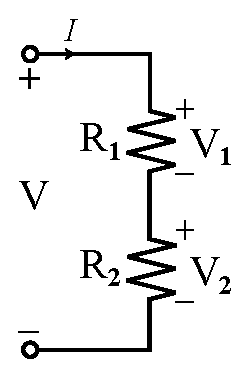
\includegraphics[width=0.3\textwidth,height=0.35\textheight]{./image/circuit1/append_end2}
\end{figure}
\begin{figure}[H]
  \centering
  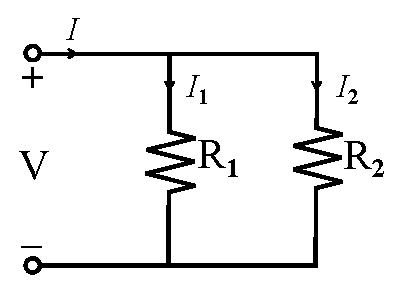
\includegraphics[width=0.6\textwidth,height=0.28\textheight]{./image/circuit1/append_end2_2}
\end{figure}
\end{column}


\end{columns}

\end{frame}
%------------------------------------------------
%------------------------------------------------

\begin{frame}
\frametitle{Solution(Q1)}
\begin{columns}
\begin{column}{6cm}
\begin{itemize} \itemsep1pt \parskip0pt \parsep0pt
  \item[Q:] \blue{Determine the resistance value of $R_1$, $R_2$,...,$R_5$ in the circuits. (Assume the resistance of $R_1$ is R)}
  \item[A:] \red{Because the resistors are in series, the resistance between successive nodes will be proportional to the voltage between the nodes.}
  \item[$\ast$] $R_1\propto V_1=1R \newline R_2\propto V_2-V_1=1R; \newline R_3\propto V_3-V_2=2R; \newline R_4\propto V_4-V_3=4R; \newline R_5\propto V_5-V_4=2R;$
\end{itemize}
\end{column}

\begin{column}{6cm}
\begin{figure}[H]
  \label{epi_circuit1}
  \centering
  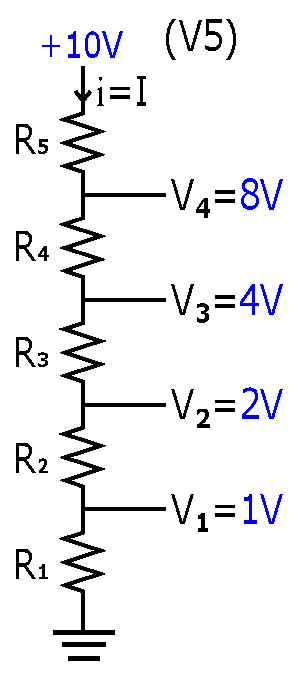
\includegraphics[width=0.45\textwidth,height=1\textwidth]{./image/circuit1/resistor1}
\end{figure}
\end{column}
\end{columns}

\end{frame}

%------------------------------------------------
%------------------------------------------------


\begin{frame}
\frametitle{Solution(Q2)}
\begin{columns}
\begin{column}{6cm}
\begin{itemize} \itemsep1pt \parskip0pt \parsep0pt
  \item[Q:] \blue{Determine $R_1$ and $R_2$}
\end{itemize}
\end{column}

\begin{column}{6cm}
\begin{figure}[H]
  \label{epi_circuit2_1}
  \centering
  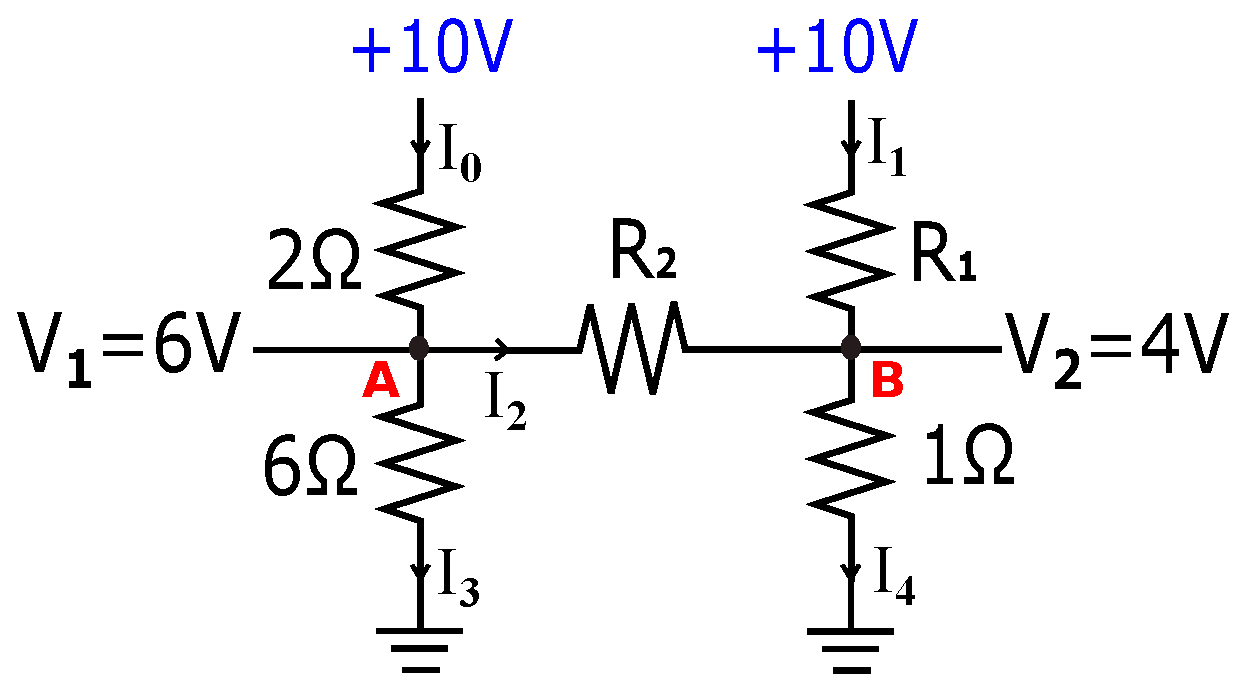
\includegraphics[width=1.0\textwidth]{./image/circuit1/circuit2_1}
\end{figure}
\end{column}
\end{columns}

\begin{itemize} \itemsep1pt \parskip0pt \parsep0pt
  \item[$\ast$]KCL at the node \red{A} determines the current \red{$I_2$} through $R_2$,(i.e. \red{$I_2 = 1A$})\item[$\ast$] To make $V_1-V_2 = 2V = I_2R_2$, it follows that \red{$R_2 = 2\Omega$}.
  \item[$\ast$]KCL at the node \red{B} then determines that \red{$I_1 = 3A$}, the current flows downward through $R_1$ .\newline To make $10V-V_2 = 6V$, it follows that \red{$R_1 = 2\Omega$}.
\end{itemize}

\end{frame}

%------------------------------------------------
%------------------------------------------------

\begin{frame}
\frametitle{Question 3}

\begin{itemize} \itemsep1pt \parskip0pt \parsep0pt
  \item \blue{If $V_{AB} = 4V$, determine $R_1$,$R_2$,$R_3$ and $R_4$}
\end{itemize}



\begin{figure}[H]
  \label{epi_circuit3}
  \centering
  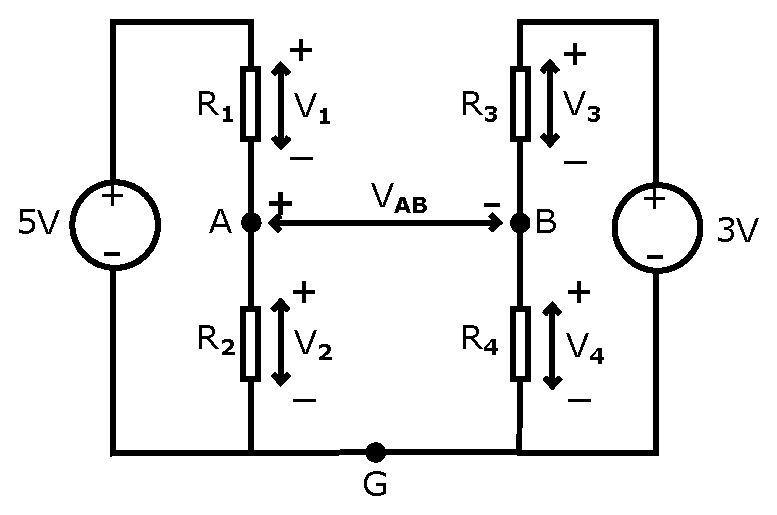
\includegraphics[width=0.6\textwidth]{./image/circuit1/circuit3}
\end{figure}


\end{frame}

%------------------------------------------------
%------------------------------------------------

\begin{frame}
\frametitle{Solution(Q3)}

\begin{columns}
\begin{column}{6cm}
\begin{itemize} \itemsep1pt \parskip0pt \parsep0pt
  \item[$\ast$] $V_{AB} = 4V$
  \item[$\ast$] If $V_B = -1.5V$, \newline then $V_A = 2.5V$

  \item[$\ast$] By potential divider, $R_1:R_2 = 1:1$, $R_3:R_4 = 1:1$
\end{itemize}
\end{column}

\begin{column}{6cm}
\begin{figure}[H]
  \label{epi_circuit3_1}
  \centering
  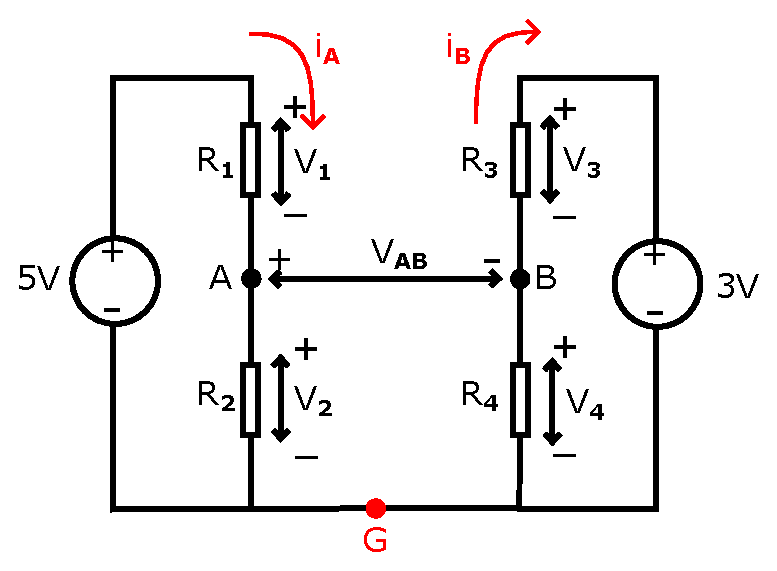
\includegraphics[width=1.0\textwidth]{./image/circuit1/circuit3_1}
\end{figure}
\end{column}
\end{columns}
\hspace{6mm} $V_A = 5\cdot \frac{R_2}{R_1+R_2}=2.5V$, $V_B = -3\cdot \frac{R_4}{R_3+R_4}=-1.5V$
\begin{itemize} \itemsep1pt \parskip0pt \parsep0pt
  \item[$\ast$] You can pick any value for resistances.
\end{itemize}
\end{frame}

%------------------------------------------------
%------------------------------------------------

\begin{frame}
\frametitle{Solution(Q3)}

\begin{columns}
\begin{column}{6cm}
\begin{itemize} \itemsep1pt \parskip0pt \parsep0pt
  \item[$\ast$] $V_{AB} = 4V$
  \item[$\ast$] If $V_B = -1V$, \newline then $V_A = 3V$
  \item[$\ast$] By potential divider, $R_1:R_2 = 2:3$, $R_3:R_4 = 2:1$
\end{itemize}
\end{column}

\begin{column}{6cm}
\begin{figure}[H]
  \label{epi_circuit3_1_1}
  \centering
  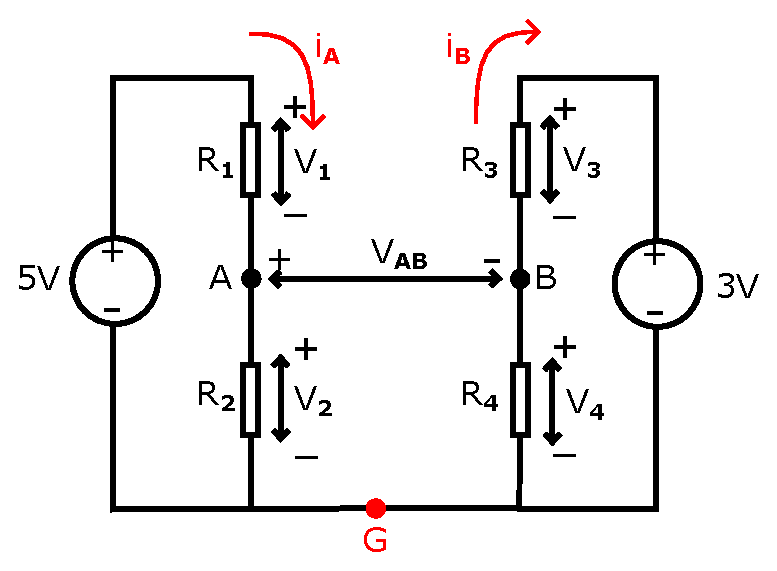
\includegraphics[width=1.0\textwidth]{./image/circuit1/circuit3_1}
\end{figure}
\end{column}
\end{columns}


\begin{itemize} \itemsep1pt \parskip0pt \parsep0pt
  \item[$\ast$] If $V_B = -2V \rightarrow V_A = 2V$\newline
  By potential divider,\newline
  $R1:R2 = 3:2$, $R3:R4 = 1:2$
\end{itemize}


\begin{itemize} \itemsep1pt \parskip0pt \parsep0pt
  \item[] \red{$V_A = 5\cdot \frac{R_2}{R_1+R_2}$, $V_B = -3\cdot \frac{R_4}{R_3+R_4}$}
  \item[] \red{$V_{AB} = V_A - V_B = \frac{5R_2}{R_1+R_2}-\frac{3R_4}{R_3+R_4}$}
\end{itemize}


\end{frame}

%------------------------------------------------
%------------------------------------------------

\begin{frame}
\frametitle{Question 4}

\begin{itemize} \itemsep1pt \parskip0pt \parsep0pt
  \item \blue{For the circuit in the figure, determine $i_1$ to $i_5$.}
\end{itemize}



\begin{figure}[H]
  \centering
  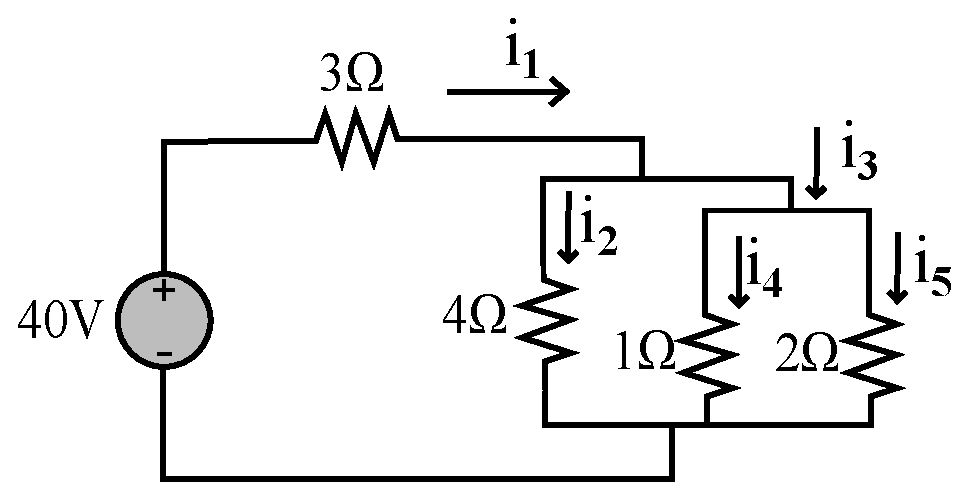
\includegraphics[width=0.6\textwidth]{./image/circuit1/circuit4}
\end{figure}


\end{frame}

%------------------------------------------------
%------------------------------------------------

\begin{frame}
\frametitle{Solution(Q4)}
\begin{itemize} \itemsep1pt \parskip0pt \parsep0pt
  	\item[$\ast$] We apply:
  	\begin{itemize} \itemsep1pt \parskip0pt \parsep0pt
  		\item[$\bullet$] $V = IR$
  		\item[$\bullet$] Series / Parallel Combinations
  		\item[$\bullet$] Current Divider
  
	\end{itemize}
\end{itemize}

\begin{columns}
\begin{column}{6cm}


\blue{$(i)$}
\begin{figure}[H]
  \label{epi_circuit4_1}
  \centering
  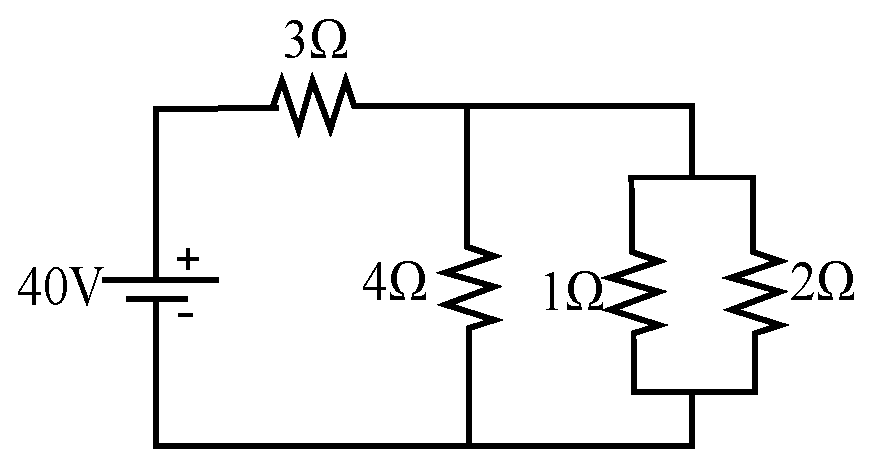
\includegraphics[width=0.8\textwidth,height=0.3\textheight]{./image/circuit1/circuit4_1}
\end{figure}
\begin{center} $1 \Omega \parallel 2 \Omega = \frac{2}{3} \Omega$\end{center}
\end{column}

\begin{column}{6cm}

\blue{$(ii)$}
\begin{figure}[H]
  \label{epi_circuit4_2}
  \centering
  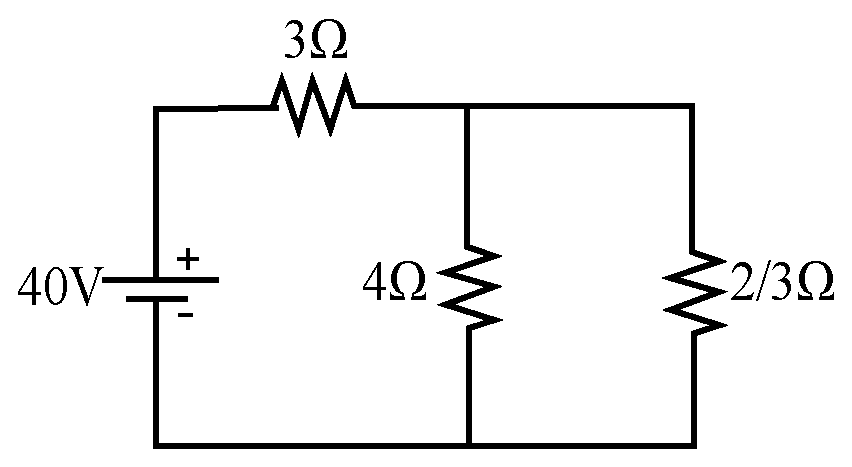
\includegraphics[width=0.8\textwidth,height=0.3\textheight]{./image/circuit1/circuit4_2}
\end{figure}
\center $4 \Omega \parallel \frac{2}{3} \Omega = \frac{4}{7} \Omega$


\end{column}
\end{columns}


\end{frame}

%------------------------------------------------
%------------------------------------------------

\begin{frame}
\frametitle{Solution(Q4)}
\begin{columns}
\begin{column}{6cm}

\blue{$(iii)$}
\begin{figure}[H]
  \label{epi_circuit4_3}
  \centering
  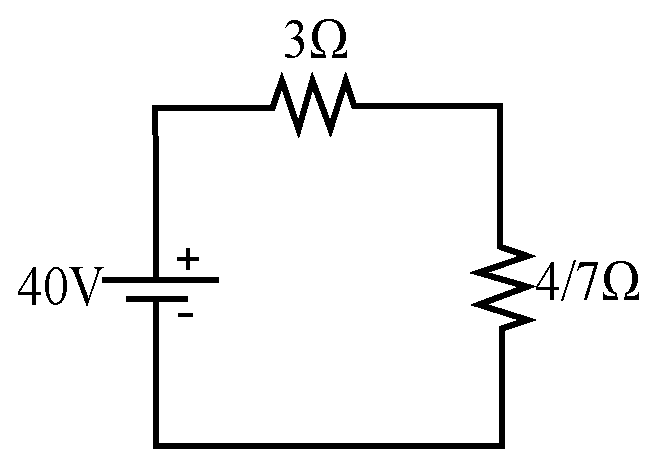
\includegraphics[width=0.8\textwidth,height=0.35\textheight]{./image/circuit1/circuit4_3}
\end{figure}
\begin{center} $3 \Omega + \frac{4}{7} \Omega = \frac{25}{7} \Omega$\end{center}
\end{column}
\begin{column}{6cm}
\begin{enumerate}[i]
  \item[$(iv)$]
\end{enumerate}
\begin{figure}[H]
  \label{epi_circuit4_4}
  \centering
  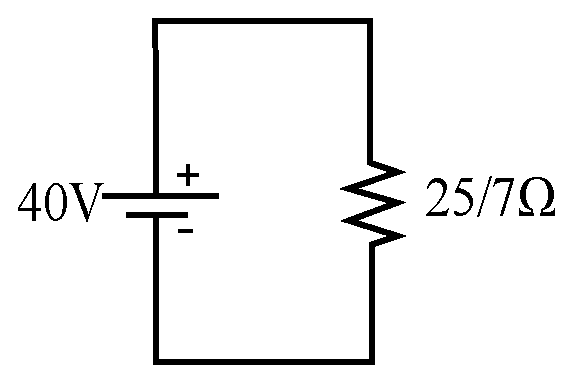
\includegraphics[width=0.8\textwidth,height=0.35\textheight]{./image/circuit1/circuit4_4}
\end{figure}
\center Simplified Circuit
\end{column}
\end{columns}
\end{frame}
%------------------------------------------------
%------------------------------------------------

\begin{frame}
\frametitle{Solution(Q4)}
\begin{columns}
\begin{column}{4cm}
\blue{$(v)$}
\begin{figure}[H]
  \label{epi_circuit4_5}
  \centering
  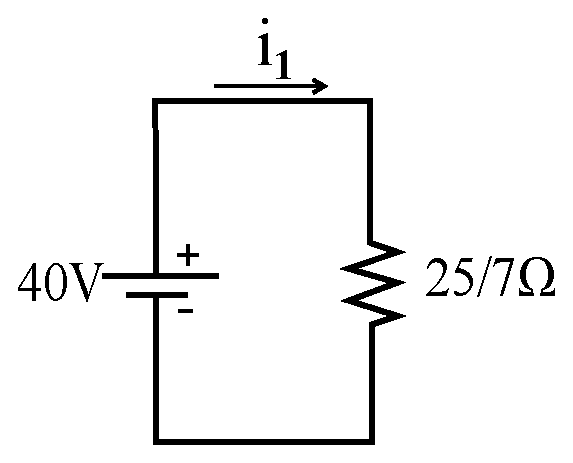
\includegraphics[width=0.9\textwidth,height=0.3\textheight]{./image/circuit1/circuit4_5}
\end{figure}
\begin{itemize} \itemsep1pt \parskip0pt \parsep0pt
  \item[$\bullet$] $V = IR$ \newline $40 = i_1 \cdot \frac{25}{7} $ \newline$\Rightarrow i_1 = 11.2A$ \newline \vspace{2 mm}
\end{itemize}
\end{column}

\begin{column}{4.3cm}
\blue{$(vi)$}
\begin{figure}[H]
  \label{epi_circuit4_6}
  \centering
  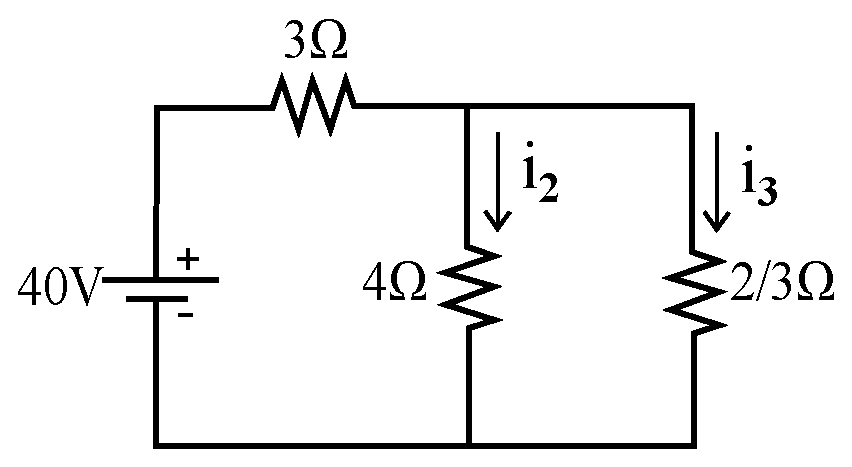
\includegraphics[width=0.9\textwidth,height=0.3\textheight]{./image/circuit1/circuit4_6}
\end{figure}
\begin{itemize} \itemsep1pt \parskip0pt \parsep0pt
  \item[$\bullet$] $i_1 = i_2 + i_3$ \newline $i_2 = \frac{\frac{2}{3}}{4+\frac{2}{3}} \cdot i_1 $\newline $= (\frac{1}{7})(11.2)=1.6A$ \newline$i_3 = 11.2-1.6 = 9.6A$
\end{itemize}
\end{column}

\begin{column}{4.3cm}
\blue{$(vii)$}
\begin{figure}[H]
  \label{epi_circuit4_7}
  \centering
  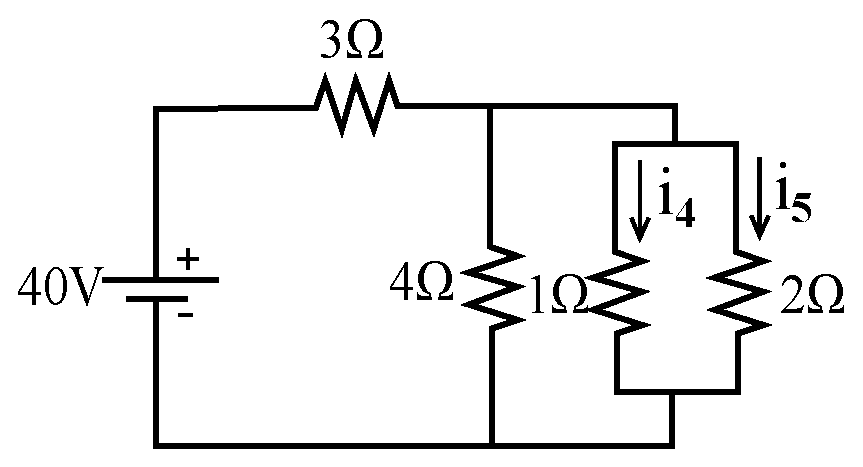
\includegraphics[width=0.9\textwidth,height=0.3\textheight]{./image/circuit1/circuit4_7}
\end{figure}
\begin{itemize} \itemsep1pt \parskip0pt \parsep0pt
  \item[$\bullet$] $i_3 = i_4 + i_5$ \newline $i_4 = (\frac{2}{3})(9.6) = 6.4A$\newline $i_5 = (\frac{1}{3})(9.6)=3.2A$ \newline \vspace{3.5 mm}
\end{itemize}
\end{column}
\end{columns}
\end{frame}
%------------------------------------------------
%------------------------------------------------

\begin{frame}
\frametitle{Question 5}


\begin{figure}[H]
  \centering
  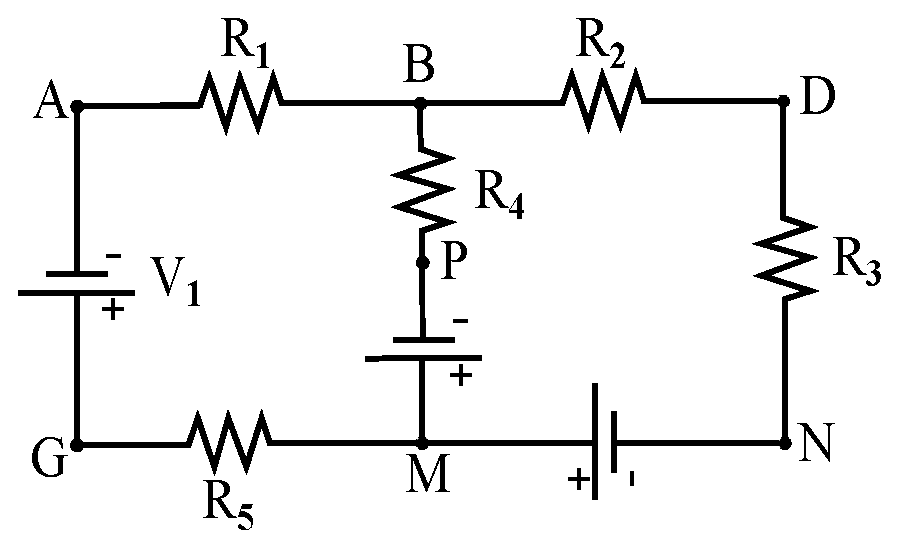
\includegraphics[width=0.6\textwidth]{./image/circuit1/circuit5}
\end{figure}


\begin{itemize} \itemsep1pt \parskip0pt \parsep0pt
  \item[$\ast$] \blue{$R_1 = 80\Omega$,$R_2 = 10\Omega$,$R_3 = 20\Omega$,$R_4 = 90\Omega$,$R_5 = 100\Omega$}
  \item[$\ast$] \blue{Battery: $V_1 = 12V$,$V_2 = 24V$,$V_3 = 36V$}
  \item[$\ast$] \blue{Resistor: $I_1$($I_5$), $I_2$($I_3$), $I_4$ = ? \hspace{8mm} $P_1$,$P_2$,...,$P_5$ = ?}
\end{itemize}


\end{frame}

%------------------------------------------------
%------------------------------------------------

\begin{frame}
\frametitle{Solution(Q5)}
\begin{columns}
\begin{column}{5cm}
\begin{itemize} \itemsep1pt \parskip0pt \parsep0pt
  \item[$\ast$]  $R_1 = 80\Omega$,$R_2 = 10\Omega$,\newline
  $R_3 = 20\Omega$,$R_4 = 90\Omega$,\newline
  $R_5 = 100\Omega$ \newline
  $V_1 = 12V$,$V_2 = 24V$,\newline
  $V_3 = 36V$
\end{itemize}
\end{column}



\begin{column}{8cm}
\begin{figure}[H]
  \centering
  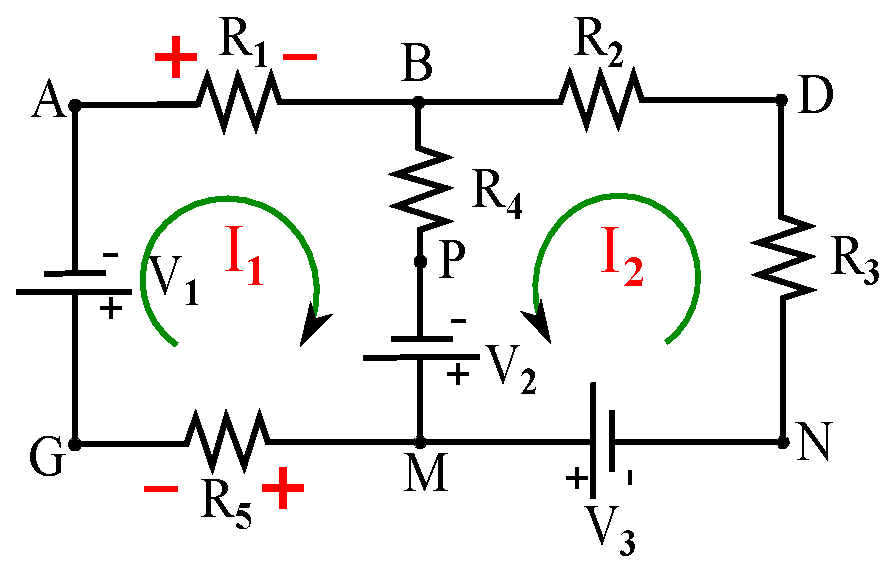
\includegraphics[width=0.9\textwidth]{./image/circuit1/circuit5_1}
\end{figure}
\end{column}
\end{columns}

\begin{itemize} \itemsep1pt \parskip0pt \parsep0pt
  \item[] {\bf Loop 1:}
  \item[$\ast$] $V_1 + I_1R_1 + (I_1+I_2)R_4 - V_2 + I_1R_5 = 0$
  \item[$\Rightarrow$] $12 + 80I_1 + 90I_1 + 90I_2 - 24 + 100I_1 = 0$
  \item[$\Rightarrow$] \red{$270I_1 + 90I_2 = 12$} \hspace{8 mm}(1)
\end{itemize}

\end{frame}

%------------------------------------------------
%------------------------------------------------

\begin{frame}
\frametitle{Solution(Q5)}
\begin{columns}
\begin{column}{5cm}
\begin{itemize} \itemsep1pt \parskip0pt \parsep0pt
  \item[$\ast$]  $R_1 = 80\Omega$,$R_2 = 10\Omega$,\newline
  $R_3 = 20\Omega$,$R_4 = 90\Omega$,\newline
  $R_5 = 100\Omega$ \newline
  $V_1 = 12V$,$V_2 = 24V$,\newline
  $V_3 = 36V$
\end{itemize}
\end{column}



\begin{column}{8cm}
\begin{figure}[H]
  \centering
  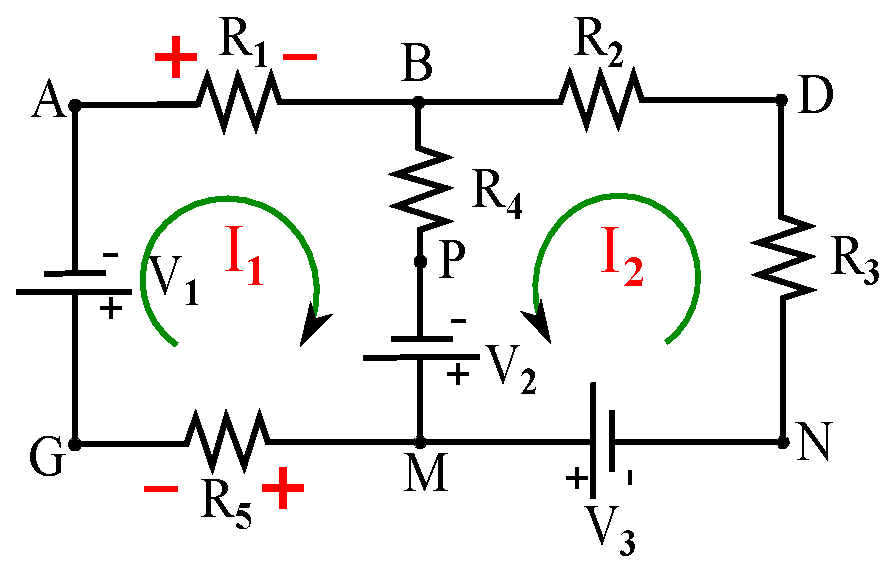
\includegraphics[width=0.9\textwidth]{./image/circuit1/circuit5_1}
\end{figure}
\end{column}
\end{columns}

\begin{itemize} \itemsep1pt \parskip0pt \parsep0pt
  \item[] {\bf Loop 2:}
  \item[$\ast$] $V_3 + I_2R_3 + I_2R_2 + (I_1 + I_2)R_4 -V_2 = 0$
  \item[$\ast$] $36 + 20I_2 + 10I_2 + 90I_1 + 90I_2- 24 = 0$
  \item[$\Rightarrow$] \red{$90I_1 + 120I_2 = -12$} \hspace{8 mm}(2)
\end{itemize}

\end{frame}

%------------------------------------------------
%------------------------------------------------

\begin{frame}
\frametitle{Solution(Q5)}
\begin{columns}
\begin{column}{5cm}
\begin{itemize} \itemsep1pt \parskip0pt \parsep0pt
  \item[$\ast$]  $R_1 = 80\Omega$,$R_2 = 10\Omega$,\newline
  $R_3 = 20\Omega$,$R_4 = 90\Omega$,\newline
  $R_5 = 100\Omega$ \newline
  $V_1 = 12V$,$V_2 = 24V$,\newline
  $V_3 = 36V$
\end{itemize}
\end{column}



\begin{column}{8cm}
\begin{figure}[H]
  \centering
  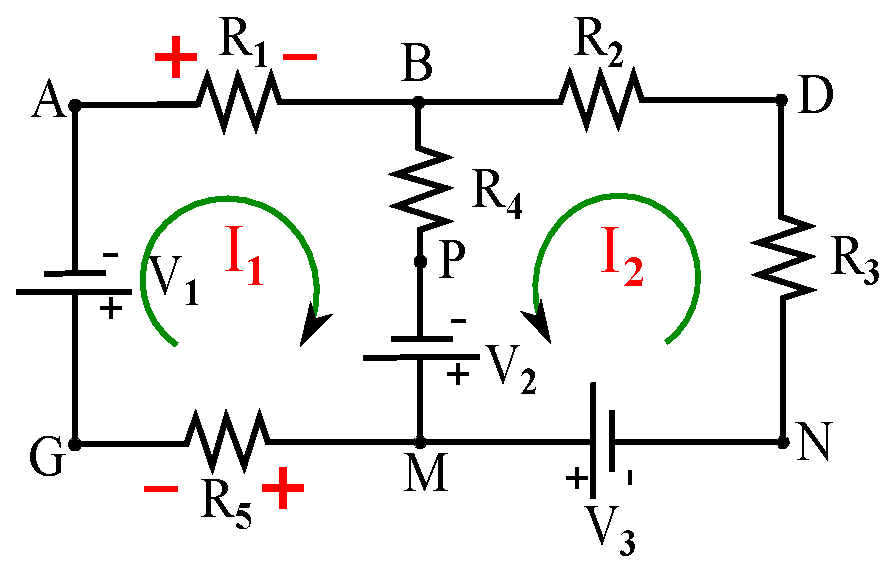
\includegraphics[width=0.9\textwidth]{./image/circuit1/circuit5_1}
\end{figure}
\end{column}
\end{columns}

\begin{itemize} \itemsep1pt \parskip0pt \parsep0pt
  \item[$\ast$] {\bf Loop 1:} $270I_1 + 90I_2 = 12$ \hspace{8 mm}(1)
  \item[$\ast$] {\bf Loop 2:} $90I_1 + 120I_2 = -12$ \hspace{8 mm}(2)
  \item[$\Rightarrow$] $I_2 = -\frac{8}{45}A$,$I_1 = \frac{14}{135}A$
\end{itemize}

\end{frame}

%------------------------------------------------
%------------------------------------------------

\begin{frame}
\frametitle{Solution(Q5)}
\begin{columns}
\begin{column}{5cm}
\begin{itemize} \itemsep1pt \parskip0pt \parsep0pt
  \item[$\ast$]  $R_1 = 80\Omega$,$R_2 = 10\Omega$,\newline
  $R_3 = 20\Omega$,$R_4 = 90\Omega$,\newline
  $R_5 = 100\Omega$ \newline
  $V_1 = 12V$,$V_2 = 24V$,\newline
  $V_3 = 36V$
\end{itemize}
\end{column}



\begin{column}{8cm}
\begin{figure}[H]
  \centering
  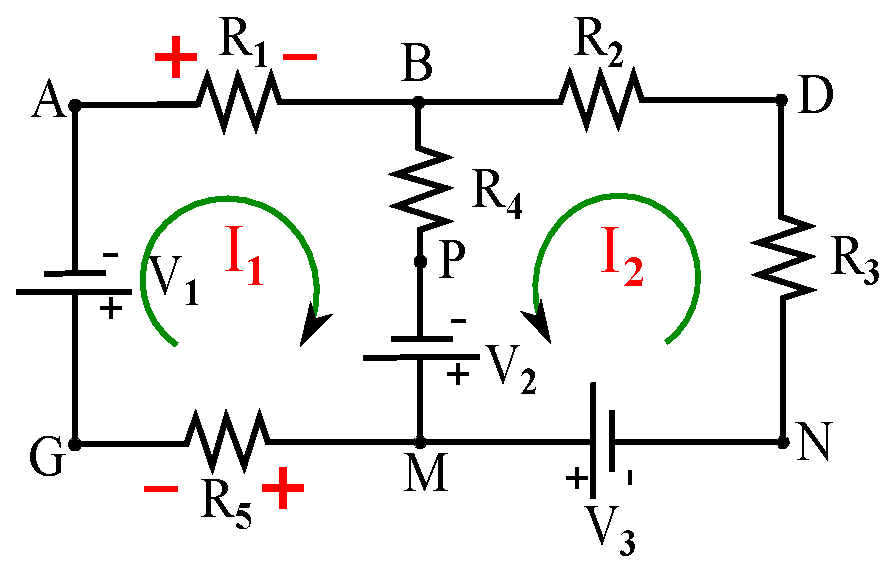
\includegraphics[width=0.9\textwidth]{./image/circuit1/circuit5_1}
\end{figure}
\end{column}
\end{columns}

\begin{itemize} \itemsep1pt \parskip0pt \parsep0pt
  \item[$\ast$] $I_1 = \frac{14}{135}A$
  \item[$\ast$] $I_2 = -\frac{8}{45}A$
  \item[$\ast$] \red{\bf{KCL of Node: $I_{R_4} = I_1 + I_2$}}
  \item[$\ast$] $P = I^2R$
  \begin{itemize} \itemsep1pt \parskip0pt \parsep0pt
    \item[$\bullet$] $P_1 = I_1^2R_1$, $P_4 = I_{R_4}^2R_4$, ...
  \end{itemize}
\end{itemize}

\end{frame}

%------------------------------------------------
%------------------------------------------------

\begin{frame}
\frametitle{Solution(Q5)}
\begin{columns}
\begin{column}{5cm}
\begin{itemize} \itemsep1pt \parskip0pt \parsep0pt
  \item[$\ast$]  $R_1 = 80\Omega$,$R_2 = 10\Omega$,\newline
  $R_3 = 20\Omega$,$R_4 = 90\Omega$,\newline
  $R_5 = 100\Omega$ \newline
  $V_1 = 12V$,$V_2 = 24V$,\newline
  $V_3 = 36V$
\end{itemize}
\end{column}



\begin{column}{8cm}
\begin{figure}[H]
  \centering
  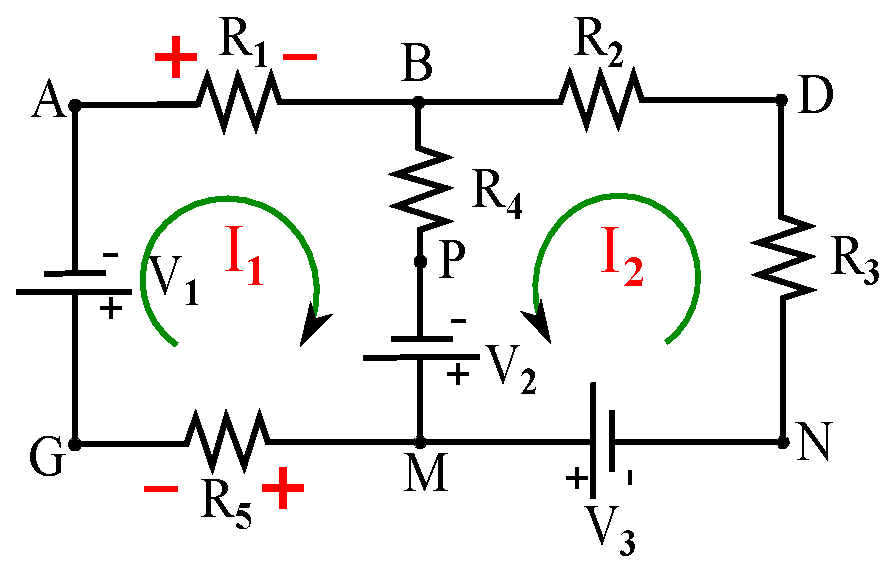
\includegraphics[width=0.9\textwidth]{./image/circuit1/circuit5_1}
\end{figure}
\end{column}
\end{columns}

\begin{itemize} \itemsep1pt \parskip0pt \parsep0pt
  \item[$\ast$] \red{$I_1 = (24 - V_B)/180 = 14/135A = 0.104A$}
  \item[$\ast$] \red{$I_4 = (12 - V_B)/90 = 2/27A = 0.074A$}
  \item[$\ast$] \red{$I_2 = -V_B/30 = -8/45A = -0.178A$}
\end{itemize}


\end{frame}

%------------------------------------------------
%------------------------------------------------

\begin{frame}
\frametitle{Solution(Q5)}
\begin{columns}
\begin{column}{5cm}
\begin{itemize} \itemsep1pt \parskip0pt \parsep0pt
  \item[$\ast$]  $R_1 = 80\Omega$,$R_2 = 10\Omega$,\newline
  $R_3 = 20\Omega$,$R_4 = 90\Omega$,\newline
  $R_5 = 100\Omega$ \newline
  $V_1 = 12V$,$V_2 = 24V$,\newline
  $V_3 = 36V$
\end{itemize}
\end{column}



\begin{column}{8cm}
\begin{figure}[H]
  \centering
  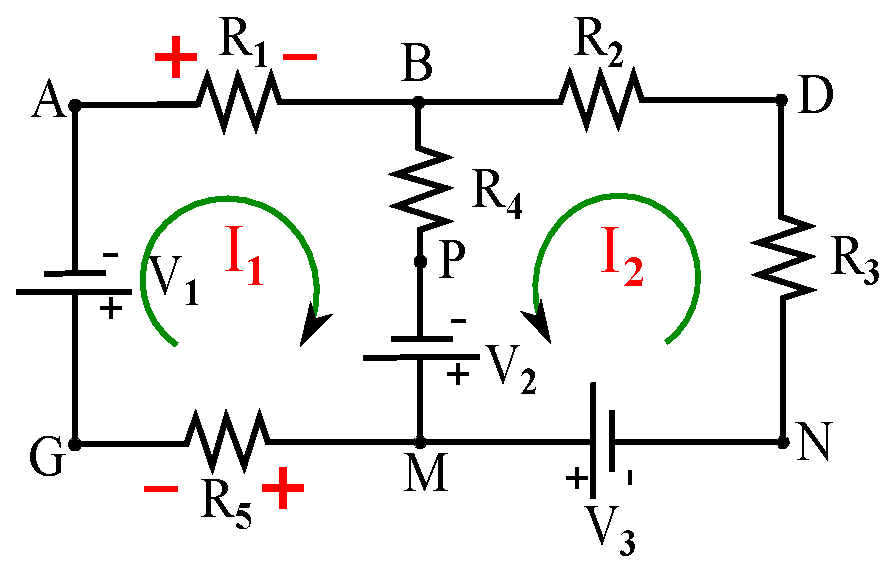
\includegraphics[width=0.9\textwidth]{./image/circuit1/circuit5_1}
\end{figure}
\end{column}
\end{columns}

\begin{itemize} \itemsep1pt \parskip0pt \parsep0pt
  \item[$\ast$] \red{$P = I^2R$, $P = V^2/R$} \blue{$\Rightarrow$} \red{$P_1 = (0.104)^2 \cdot 80 = 0.86528W$}
  \item[$\ast$] \red{$P_2 = (-0.178)^2 \cdot 10 = 0.31684W$}
  \item[$\ast$] \red{$P_4 = (0.074)^2 \cdot 90 = 0.49284W = {V_{R_4}}^2/R_4$}
  \item[$\ast$] \red{$P_3 = (-0.178)^2 \cdot 20 = 0.63368W$}
  \item[$\ast$] \red{$P_5 = (0.104)^2 \cdot 100 = 1.0816W$}
\end{itemize}

\end{frame}

%------------------------------------------------
%------------------------------------------------

\begin{frame}
\frametitle{Question 6}
\begin{columns}

\begin{column}{6cm}
\begin{itemize} \itemsep1pt \parskip0pt \parsep0pt
  \item[$\ast$] \blue{You have connected the lamp, with $V_{cc} = 12V$. The datasheet of the lamp states that it only turns on when $V_L > 8V$. The lamp has an internal resistance of $1k \Omega$.}
  \item[$\ast$] \blue{What is the range of $R$ that would allow the circuit to function correctly with all input combinations.}
\end{itemize}
\end{column}


\begin{column}{6cm}
\begin{figure}[H]
  \centering
  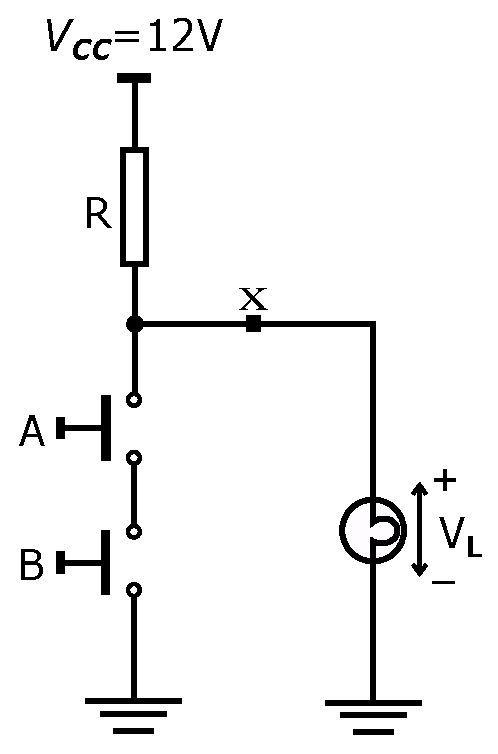
\includegraphics[width=0.6\textwidth]{./image/circuit1/circuit6}
\end{figure}
\end{column}

\end{columns}

\end{frame}

%------------------------------------------------
%------------------------------------------------

\begin{frame}
\frametitle{Solution(Q6)}

\begin{columns}

\begin{column}{6cm}
\begin{itemize} \itemsep1pt \parskip0pt \parsep0pt
  \item[$\ast$] The range of R
  \item[$\ast$] When the lamp is turned on, \red{$x =$ ``1''}, $V_L > 8$ \newline$12 \times \frac{R_L}{R_L + R} > 8 \Rightarrow R < 500 \Omega$
  \item[$\ast$] When the lamp is off, \red{$x =$ ``0''}, and $V_L < 8$. It will function regardless of the value of $R$.
\end{itemize}
\end{column}


\begin{column}{6cm}
\begin{figure}[H]
  \centering
  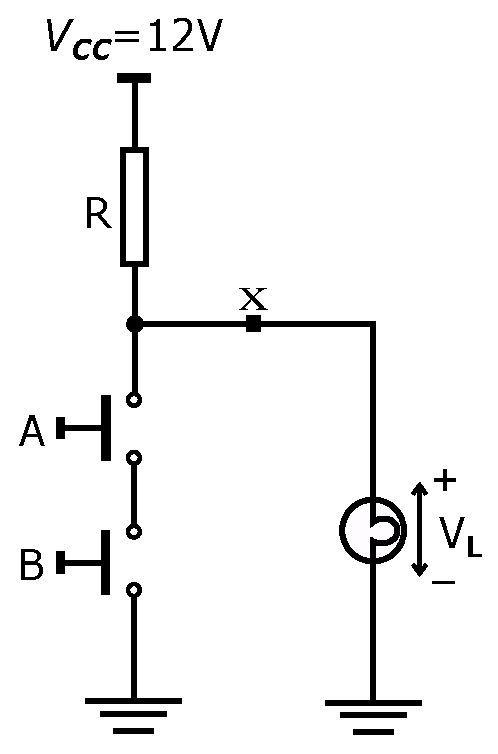
\includegraphics[width=0.6\textwidth]{./image/circuit1/circuit6}
\end{figure}
\end{column}

\end{columns}

\end{frame}

%------------------------------------------------
%------------------------------------------------

\begin{frame}
\frametitle{Question 7a}
\begin{itemize} \itemsep1pt \parskip0pt \parsep0pt
  \item[$\ast$] A force sensitive resistor (FSR) is a resistor with its resistance changed according to the force applied to it.
\end{itemize}

\begin{columns}

\begin{column}{6cm}
\begin{itemize} \itemsep1pt \parskip0pt \parsep0pt
  \item[$\ast$] For simplicity sake, your partner has wired up the FSR using a simple potential divider circuit
\end{itemize}
\begin{table}
\begin{center}
\def\arraystretch{1.5}
\begin{tabular}{|c||c|}
\hline
Force (N) & Resistance $R_{fsr} (\Omega)$ \\
\hline
0     & \bf{1M}\\
\hline
0.5   & \bf{10k}\\
\hline
1     & \bf{6k}\\
\hline
10    & \bf{1k}\\
\hline
\end{tabular}
\end{center}
\end{table}

\end{column}


\begin{column}{6cm}
\begin{figure}[H]
  \centering
  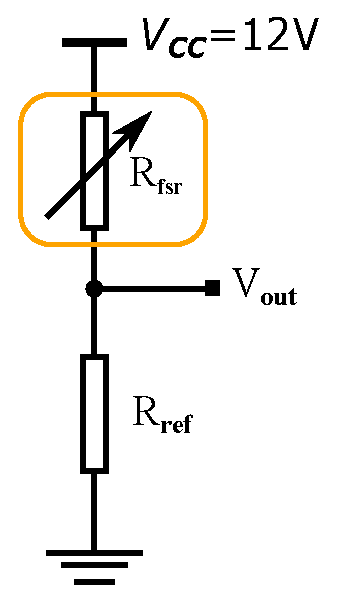
\includegraphics[width=0.45\textwidth,height=0.55\textheight]{./image/circuit1/circuit7}
\end{figure}
\end{column}

\end{columns}

\end{frame}

%------------------------------------------------
%------------------------------------------------

\begin{frame}
\frametitle{Solution(Q7a)}
\begin{itemize} \itemsep1pt \parskip0pt \parsep0pt
  \item[$\ast$] Calculate the following quantities when $R_{ref} = 10k \Omega$:
  \begin{itemize} \itemsep1pt \parskip0pt \parsep0pt
  \item[$\bullet$] Voltage across the FSR;
  \item[$\bullet$] Voltage at $V_{out}$;
  \item[$\bullet$] Current going through the FSR.
  \end{itemize}
\end{itemize}

\begin{columns}

\begin{column}{6cm}

\begin{table}
\begin{center}
\def\arraystretch{1.5}
\begin{tabular}{|c|c|c|c|}
\hline
$R_{fsr}$ & $I_{fsr}$ & $V_{fsr}$ & $V_{out}$ \\
\hline
$1M$    & $11.9 \mu A$ & $11.9V$ & $0.1V$ \\
\hline
$10k$   & $0.6mA$ & $6V$ & $6V$ \\
\hline
$6k$    & $0.75mA$ & $4.5V$ & $7.5V$ \\
\hline
$1k$    & $1.09mA$ & $1.09V$ & $10.91V$ \\
\hline
\end{tabular}
\end{center}
\end{table}

\end{column}


\begin{column}{6cm}
\begin{figure}[H]
  \centering
  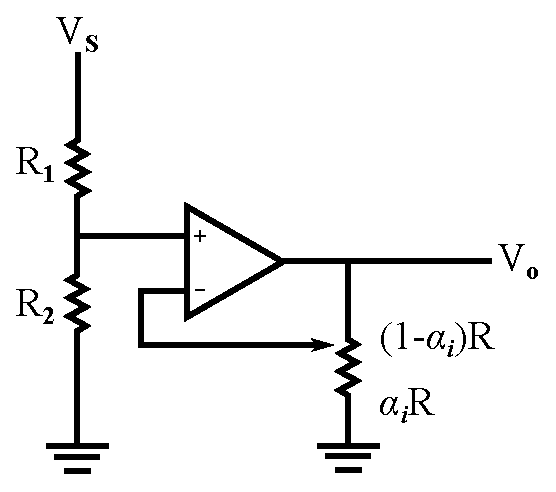
\includegraphics[width=0.4\textwidth,height=0.5\textheight]{./image/circuit1/circuit7_1}
\end{figure}
\end{column}

\end{columns}

\end{frame}

%------------------------------------------------
%------------------------------------------------

\begin{frame}
\frametitle{Question 7b}
\begin{itemize} \itemsep1pt \parskip0pt \parsep0pt
  \item[$\ast$] The output $V_{out}$ is used to detect the presence of a ball. Due to its light weight, the ball produces only 0.5N when it is located on top of the sensor. The rest of the system requires that $V_{IL} = 2V$ and $V_{IH} = 10V$
  \begin{itemize} \itemsep1pt \parskip0pt \parsep0pt
  \item[$\bullet$] $V_{IL}$: Max. voltage that the system regards as logical LOW
  \item[$\bullet$] $V_{IH}$: Min. voltage that the system regards as logical HIGH
  \end{itemize}

  \item[$\ast$] Determine the range of value that $R_{ref}$ may take for correct functioning of the circuit.
  \begin{itemize} \itemsep1pt \parskip0pt \parsep0pt
  \item[$\bullet$] It should output a logical HIGH when a ball is presence and a logical LOW otherwise.
  \end{itemize}
\end{itemize}
\begin{columns}


\end{columns}

\end{frame}

%------------------------------------------------
%------------------------------------------------

\begin{frame}
\frametitle{Solution(Q7b)}
\begin{columns}

\begin{column}{2cm}
\begin{figure}[H]
  \centering
  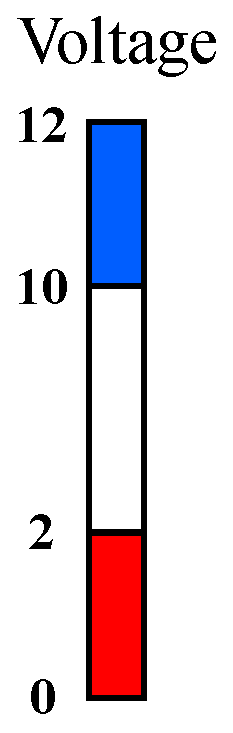
\includegraphics[width=1\textwidth]{./image/circuit1/circuit7_2b}
\end{figure}
\end{column}

\begin{column}{7cm}
\vspace{10 mm}
\begin{itemize} \itemsep1pt \parskip0pt \parsep0pt
  \item[$\leftarrow$] $V_{CC} = 12V$ \vspace{2 mm}
  \item[$\leftarrow$](Presence of the ball / 0.5N)\vspace{2 mm}
  \item[$\leftarrow$] $V_{IH} = 10V$; Minimum HIGH \newline$R_{fsr} = R_H = 10k\Omega$ \vspace{4 mm}
  \item[$\leftarrow$] $10V$ -- $2V$: (Unknown; Not in use)\vspace{8 mm}
  \item[$\leftarrow$] $V_{IL} = 2V$; Maximum LOW\vspace{3 mm}
  \item[$\leftarrow$] (Absence of the ball / 0N)\vspace{3 mm}
  \item[$\leftarrow$] $V_{GND} = 0V$
\end{itemize}
\end{column}

\begin{column}{4cm}
\begin{figure}[H]
  \centering
  \includegraphics[width=0.5\textwidth]{./image/circuit1/circuit7_2}
\end{figure}
\vspace{20 mm}
\end{column}







\end{columns}

\end{frame}

%------------------------------------------------
%------------------------------------------------

\begin{frame}
\frametitle{Solution(Q7b)}
\begin{itemize} \itemsep1pt \parskip0pt \parsep0pt
  \item[$\ast$] When the ball is on the sensor, $R_{fsr} = R_H = 10k\Omega$. The output voltage at that time should be higher than $V_{IH}$.
  \item[$\ast$] When the ball is not on the sensor, then $R_{fsr} = R_L = 1M\Omega$. The output voltage should be lower than $V_{IL}$.
\end{itemize}

\begin{columns}

\begin{column}{4cm}
\begin{figure}[H]
  \centering
  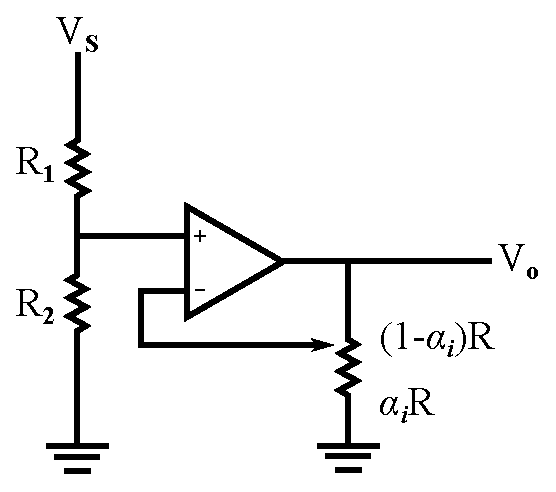
\includegraphics[width=0.6\textwidth,height=0.55\textheight]{./image/circuit1/circuit7_1}
\end{figure}
\end{column}


\begin{column}{8.5cm}

$
\begin{cases} 
V_{IH} < 12 \cdot \frac{R_{ref}}{R_H + R_{ref}} \\
12 \cdot \frac{R_{ref}}{R_H + R_{ref}} < V_{IL}
\end{cases}
$
$\Rightarrow$
$\begin{cases} 
V_{IH} < 12 \cdot \frac{R_{ref}}{R_H + R_{ref}} \\
12 \cdot \frac{R_{ref}}{R_H + R_{ref}} < V_{IL}
\end{cases}
$

\vspace{6 mm}
$\Rightarrow 50k\Omega < R_{ref} < 200k\Omega$
\end{column}
\end{columns}

\end{frame}

%------------------------------------------------
%------------------------------------------------

\begin{frame}
\frametitle{Question 7c}
\begin{itemize} \itemsep1pt \parskip0pt \parsep0pt
  \item[$\ast$] Your partner suggests that it may be possible to use 2 FSRs connected to perform a logical OR operation: When the ball rolls over either one of the 2 FSRs, the output $V_{out}$ is HIGH, and is LOW otherwise.


\end{itemize}
\begin{columns}
\begin{column}{8.5cm}
\begin{itemize} \itemsep1pt \parskip0pt \parsep0pt
  \item[$\ast$] What is the output voltage $V_{out}$?
  \begin{itemize} \itemsep1pt \parskip0pt \parsep0pt
  \item[$\bullet$] one of the FSRs is under pressure of 0.5N;
  \item[$\bullet$] both FSRs are under a pressure of 0.5N each;
  \item[$\bullet$] none of the FSRs is under pressure;
  \item[] \red{(assume $R_{ref}$ is $100k \Omega$)}
  \end{itemize}
\end{itemize}
\end{column}


\begin{column}{4cm}
\begin{figure}[H]
  \centering
  \includegraphics[width=0.9\textwidth,height=0.55\textheight]{./image/circuit1/circuit7_2}
\end{figure}
\end{column}



\end{columns}

\end{frame}

%------------------------------------------------
%------------------------------------------------

\begin{frame}
\frametitle{Solution(Q7c)}
\begin{itemize} \itemsep1pt \parskip0pt \parsep0pt
  \item[$\ast$] If $R_{ref} = 100k \Omega$,
  \begin{itemize} \itemsep1pt \parskip0pt \parsep0pt
  \item[$\bullet$] $(i)$ one of the FSRs is under pressure of 0.5N;
  \item[$\bullet$] $(ii)$ both FSRs are under a pressure of 0.5N each;
  \item[$\bullet$] $(iii)$ none of the FSRs is under pressure;
  \item[$\bullet$] $R_{eqv}$ is the equivalent resistance of the parallel combination of the two FSRs.
  \end{itemize}
\end{itemize}
\begin{columns}
\begin{column}{8.5cm}
\begin{table}
\begin{tabular}{l l l l l}
\toprule
\textbf{Case} & \textbf{$R_{fsr1}(\Omega)$} & \textbf{$R_{fsr2}(\Omega)$} & \textbf{$R_{eqv}(\Omega)$} & \textbf{$V_{out}(V)$}\\
\midrule
(i)   & 10000   & 1000000 & 9901   & \red{{\bf 10.9}} \\
(ii)  & 10000   & 10000   & 5000   & \red{{\bf 11.4}} \\
(iii) & 1000000 & 1000000 & 500000 & \red{{\bf 2}} \\
\bottomrule
\end{tabular}

\end{table}

\end{column}


\begin{column}{4cm}
\begin{figure}[H]
  \centering
  \includegraphics[width=0.75\textwidth,height=0.4\textheight]{./image/circuit1/circuit7_2}
\end{figure}
\end{column}


\end{columns}

\end{frame}

%------------------------------------------------
%------------------------------------------------

\begin{frame}
\frametitle{Question 7d}

\begin{columns}
\begin{column}{8.5cm}
\begin{itemize} \itemsep1pt \parskip0pt \parsep0pt
  \item[$\ast$] Recall that $V_{IL}$ is $2V$ and $V_{IH}$ is $10V$, is the circuit functioning correctly as a 2-input OR?
  \vspace{8mm}
  \item[$\ast$] If there are 3 FSRs connected in parallel, assumer $R_{ref}$ remains at 100k, will the circuit behave as a 3-input OR?
\end{itemize}
\end{column}


\begin{column}{4cm}
\begin{figure}[H]
  \centering
  \includegraphics[width=0.9\textwidth,height=0.55\textheight]{./image/circuit1/circuit7_2}
\end{figure}
\end{column}



\end{columns}

\end{frame}

%------------------------------------------------
%------------------------------------------------

\begin{frame}
\frametitle{Solution(Q7d)}

\begin{columns}
\begin{column}{3cm}
\begin{figure}[H]
  \centering
  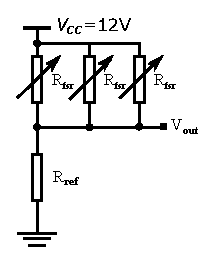
\includegraphics[width=1\textwidth,height=0.5\textheight]{./image/circuit1/circuit7_3}
\end{figure}
\end{column}

\begin{column}{8cm}
\begin{itemize} \itemsep1pt \parskip0pt \parsep0pt
  \item[$\ast$] {\bf Yes}, it works correctly as a 2-input OR gate because the output is HIGH when there is a ball on top of at least one of the input.
  \item[$\ast$] However, even if we connect 3 FSRs in parallel, the circuit cannot correctly function as a 3-input OR gate. In the case when there is \red{{\bf no ball}} falling on the circuit, the \red{{\bf equivalent resistance}} of the parallel combination of the 3 FSRs \red{{\bf drops too low}} that $V_{out} > 2V$ . As a result, the output fails to represent a logical LOW in this case.
\end{itemize}
\end{column}



\end{columns}

\end{frame}

%------------------------------------------------
%------------------------------------------------

\begin{frame}
\frametitle{Solution(Q7d)}

\begin{columns}
\begin{column}{3cm}
\begin{figure}[H]
  \centering
  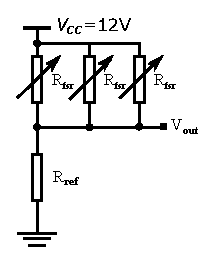
\includegraphics[width=1\textwidth,height=0.5\textheight]{./image/circuit1/circuit7_3}
\end{figure}
\end{column}

\begin{column}{8cm}

\begin{table}
\begin{tabular}{l l l l l}
\toprule
\textbf{$R_{fsr1}$} & \textbf{$R_{fsr2}$} & \textbf{$R_{fsr3}$} & \textbf{$R_{eqv}$} & \textbf{$V_{out}$}\\
\midrule
1000000   & 1000000   & 1000000 & 333333.33   & {\bf 2.77}  \\
1000000   & 1000000   & 10000   & 9803.92     & 10.93 \\
1000000   & 10000     & 1000000 & 9803.92     & 10.93 \\
1000000   & 10000     & 10000   & 4975.12     & 11.43 \\
10000     & 1000000   & 1000000 & 9803.92     & 10.93 \\
10000     & 1000000   & 10000   & 4975.12     & 11.43 \\
10000     & 10000     & 1000000 & 4975.12     & 11.43 \\
10000     & 10000     & 10000   & 3333.33     & 11.61 \\
\bottomrule
\end{tabular}

\end{table}
\end{column}



\end{columns}

\end{frame}

%------------------------------------------------

%------------------------------------------------

\begin{frame}
\frametitle{Appendix(Question)}
\begin{columns}
\begin{column}{4.5cm}
\blue{\bf Wheatstone bridge}

\begin{figure}[H]
  \centering
  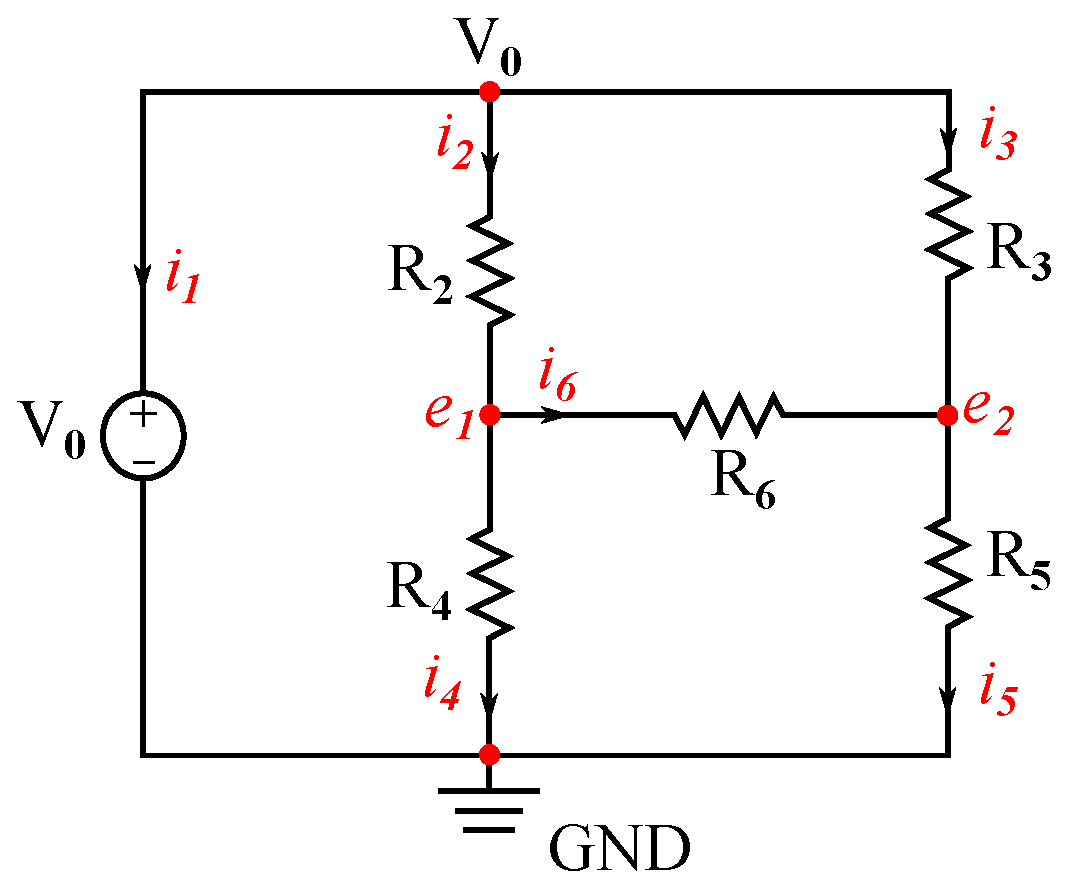
\includegraphics[width=1\textwidth,height=0.5\textheight]{./image/circuit1/circuit_q}
\end{figure}
\end{column}


\begin{column}{8cm}
\begin{table}
\begin{center}
\def\arraystretch{1.5}

\begin{tabular}{|c|c|c|}
\hline
{} & NOT Always & Always \\ {} & True & True \\ 
\hline
If $\frac{R_2}{R_4} = \frac{R_3}{R_5}$, & {} & {} \\ 
then $i_6 = 0$    & {} & {} \\
\hline
$i_2 + i_3 = i_4 + i_5$  & {} & {} \\
\hline
$i_2 + i_6 = i_3$   & {} & {} \\
\hline
$e_1 = \frac{R_4}{R_2 + R_4}V_0$    & {} & {} \\
\hline
If $i_6 = 0$, then & {} & {} \\ $\frac{R_2}{R_2 + R_4} = \frac{R_3}{R_3 + R_5}$    & {} & {} \\
\hline
\end{tabular}
\end{center}
\end{table}


\end{column}
\end{columns}
\end{frame}

%------------------------------------------------
%------------------------------------------------

\begin{frame}
\frametitle{Appendix(Solution)}

\begin{table}
\begin{center}
\def\arraystretch{1.5}

\begin{tabular}{|c|c|c|}
\hline
{} & NOT Always True & Always True \\
\hline
If $\frac{R_2}{R_4} = \frac{R_3}{R_5}$, & {} & {} \\ 
then $i_6 = 0$    & {} & \huge{\checkmark} \\
\hline
$i_2 + i_3 = i_4 + i_5$  & {} & \huge{\checkmark} \\
\hline
$i_2 + i_6 = i_3$   & \huge{\checkmark} & {} \\
\hline
$e_1 = \frac{R_4}{R_2 + R_4}V_0$    & \huge{\checkmark} & {} \\
\hline
If $i_6 = 0$, then & {} & {} \\ $\frac{R_2}{R_2 + R_4} = \frac{R_3}{R_3 + R_5}$    & {} & \huge{\checkmark} \\
\hline
\end{tabular}
\end{center}
\end{table}


\end{frame}

%------------------------------------------------
%------------------------------------------------

\begin{frame}
\frametitle{Appendix(Question 8)}

\begin{itemize} \itemsep1pt \parskip0pt \parsep0pt
  \item[$\ast$] Find $V_2$ using single loop analysis
  \begin{itemize} \itemsep1pt \parskip0pt \parsep0pt
    \item[$\bullet$] Without simplifying the circuit
    \item[$\bullet$] Simplifying the circuit
  \end{itemize}
\end{itemize}
\vspace{8 mm}

$V_{s1} = 2V, V_{s2} = 2V, V_{s3} = 2V, R_1 = 1\Omega, R_2 = 2\Omega, R_3 = 4\Omega$


\begin{figure}[H]
  \centering
  \includegraphics[width=0.6\textwidth,height=0.45\textheight]{./image/circuit1/circuit8}
\end{figure}


\end{frame}

%------------------------------------------------
%------------------------------------------------

\begin{frame}
\frametitle{Appendix(Solution(Q8))}
\blue{{\bf Without Simplifying the circuit}}

\begin{columns}
\begin{column}{7cm}
\begin{itemize} \itemsep1pt \parskip0pt \parsep0pt
  \item[$\ast$] Choose loop current
  \item[$\ast$] Apply KVL
  \begin{itemize} \itemsep1pt \parskip0pt \parsep0pt
    \item[$\bullet$] Replace $V_2$ by $R_2I$
    \item[$\bullet$] $+V_{s2} + R_1I +$\red{$ R_2I$}$ + R_3I + V_{s3} - V_{s1} = 0$
    \item[$\Rightarrow$] $I = -\frac{2}{7}A$
  \end{itemize}
  \item[$\ast$] Find $V_2$
  \begin{itemize} \itemsep1pt \parskip0pt \parsep0pt
    \item[$\bullet$] $V_2 = -R_2I = \frac{4}{7}V$
  \end{itemize}
  \vspace{8 mm}
  \item[] \orange{{\bf Notice: Ignore sign symbols(+/-) on resistor when calculating currents($R_2$ in this example!!!)}}
\end{itemize}
\end{column}

\begin{column}{5cm}
\begin{figure}[H]
  \centering
  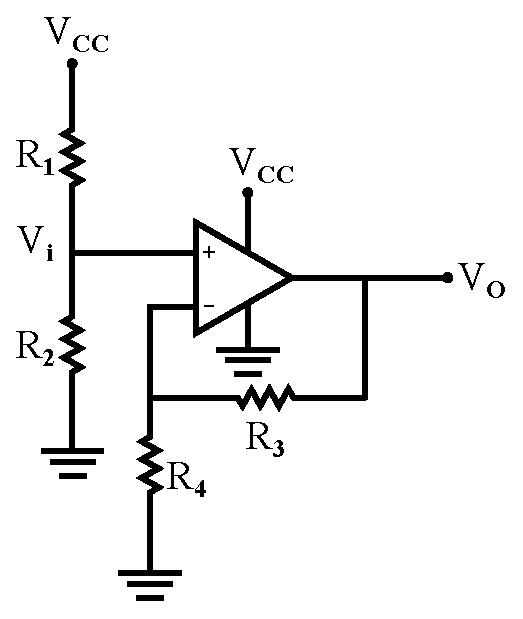
\includegraphics[width=1\textwidth,height=0.4\textheight]{./image/circuit1/circuit8_1}
\end{figure}
\end{column}



\end{columns}


\end{frame}

%------------------------------------------------
%------------------------------------------------

\begin{frame}
\frametitle{Appendix(Solution(Q8))}
\blue{{\bf Simplifying the circuit}}

\begin{columns}
\begin{column}{7cm}
\begin{itemize} \itemsep1pt \parskip0pt \parsep0pt
  \item[$\ast$] Simplifying the circuit with one voltage source and one resistor
  \item[$\ast$] $R_{eq} = R_1 + R_2 + R_3 = 7\Omega$
  \item[$\ast$] $V_{eq} = V_{s1} + V_{s2} + V_{s3} = -2 + 2 + 2 = 2V$
  \item[$\Rightarrow$] $I = V_{eq}/V_{eq} = \frac{2}{7}A$
  \item[$\Rightarrow$] $V_2 = \frac{4}{7}V$
\end{itemize}
\end{column}

\begin{column}{5cm}
\begin{figure}[H]
  \centering
  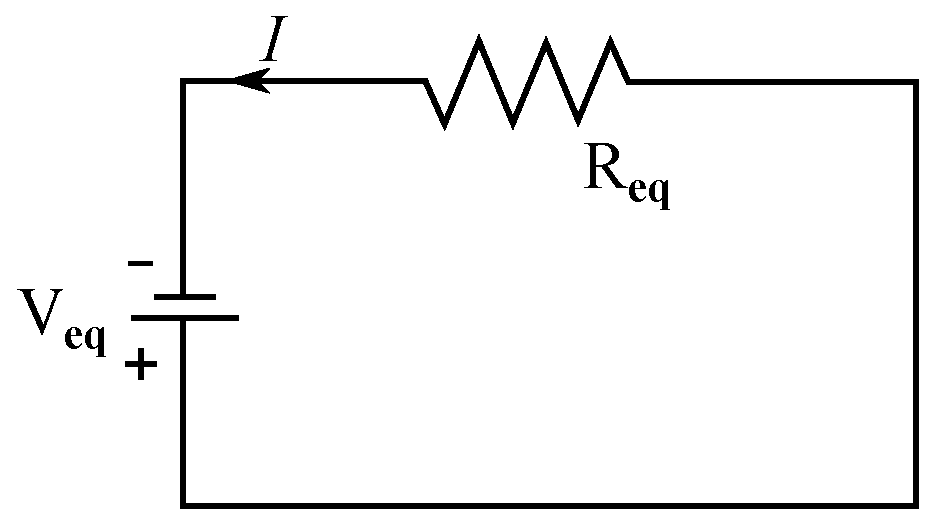
\includegraphics[width=1\textwidth,height=0.4\textheight]{./image/circuit1/circuit8_2}
\end{figure}
\end{column}



\end{columns}


\end{frame}

%------------------------------------------------
%------------------------------------------------
\begin{frame}
\frametitle{Appendix(Question 9)}
\begin{itemize} \itemsep1pt \parskip0pt \parsep0pt
  \item[$\ast$] Find $R_{eq}$ and $i_o$ in the circuit of the figure.
\end{itemize}

\begin{figure}[H]
  \centering
  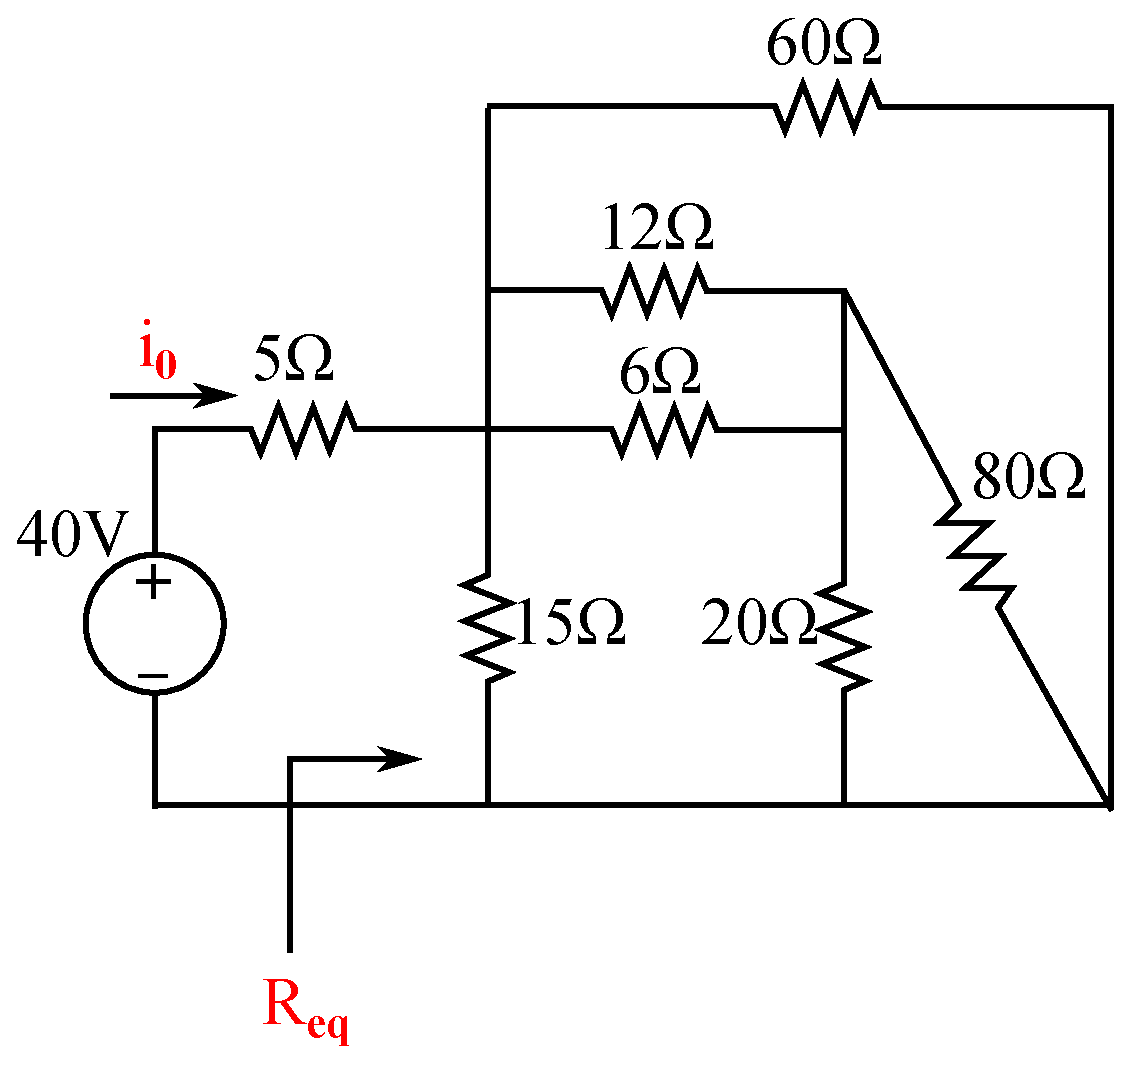
\includegraphics[width=0.6\textwidth,height=0.75\textheight]{./image/circuit1/circuit9}
\end{figure}


\end{frame}
%------------------------------------------------
%------------------------------------------------

\begin{frame}
\frametitle{Appendix(Solution(Q9))}


\begin{columns}
\begin{column}{8cm}
\begin{figure}[H]
  \includegraphics[width=0.6\textwidth,height=0.36\textheight]{./image/circuit1/circuit9_1}
\end{figure}

\begin{figure}[H]
  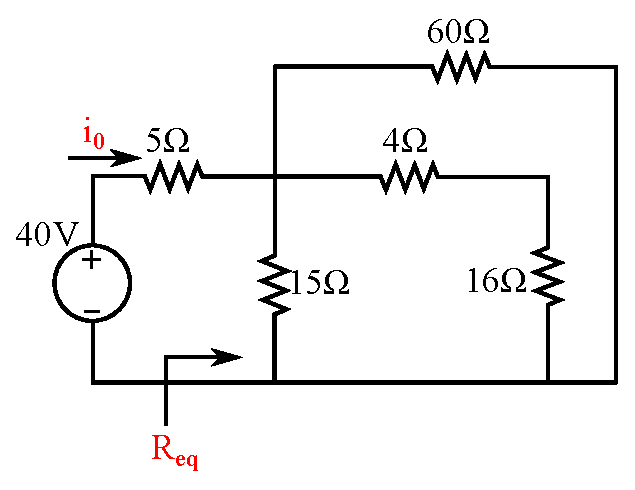
\includegraphics[width=0.6\textwidth,height=0.36\textheight]{./image/circuit1/circuit9_2}
\end{figure}
\end{column}

\begin{column}{4cm}
\begin{itemize} \itemsep1pt \parskip0pt \parsep0pt
  \item[] \blue{\bf $12\Omega \parallel 6\Omega = 4\Omega$}
  \item[] \blue{\bf $20\Omega \parallel 80\Omega = 16\Omega$}
\end{itemize}
\vspace{30 mm}
\begin{itemize} \itemsep1pt \parskip0pt \parsep0pt
  \item[] \blue{\bf $4\Omega + 16\Omega = 20\Omega$}
\end{itemize}
\vspace{6 mm}
\end{column}



\end{columns}


\end{frame}

%------------------------------------------------
%------------------------------------------------

\begin{frame}
\frametitle{Appendix(Solution(Q9))}


\begin{columns}
\begin{column}{6cm}
\begin{figure}[H]
  \includegraphics[width=0.75\textwidth,height=0.36\textheight]{./image/circuit1/circuit9_3}
\end{figure}

\end{column}

\begin{column}{6cm}
\begin{itemize} \itemsep1pt \parskip0pt \parsep0pt
  \item[] \blue{\bf $R_{eq} = 15 \parallel 20 \parallel 60\Omega = 7.5\Omega$}
  \item[] \blue{\bf $V = IR \Rightarrow 40 = i_0 \cdot 7.5 + 5 \Rightarrow i_0 = 3.2A$}
\end{itemize}

\end{column}



\end{columns}


\end{frame}

%------------------------------------------------







%------------------------------------------------
\begin{frame}
\frametitle{Appendix(Rules Governing Currents and Voltages)}
\begin{block}{Rule 1: Currents flow in loops}
The same amount of current flows into the bulb (top path) and out of the bulb (bottom path)
\end{block}

\begin{block}{Rule 2: Like the flow of water, the flow of electrical
current (charged particles) is incompressible}
Kirchoff’s Current Law (KCL): the sum of the currents into a node is zero
\end{block}

\begin{block}{Rule 3: Voltages accumulate in loops}
Kirchoff’s Voltage Law (KVL): the sum of the voltages around a closed loop is zero
\end{block}
\end{frame}

%------------------------------------------------
%------------------------------------------------
\begin{frame}
\frametitle{Appendix(Analyzing Circuits)}
\begin{itemize} \itemsep1pt \parskip0pt \parsep0pt
  	\item[$\bullet$] Assign \red{node voltage variables} to every node except ground (whose voltage is arbitrarily taken as zero)
  	\item[$\bullet$] Assign \red{component current variables} to every component in the circuit
  	\item[$\bullet$] Write one \red{constructive relation} for each component in terms of the component current variable and the component voltage
  	\item[$\bullet$] Express \red{KCL} at each node except ground in terms of the component currents
  	\item[$\bullet$] \red{Solve} the resulting equations
	\item[$\bullet$] $Power = IV = I^2R = V^2/R$
\end{itemize}
\end{frame}

%------------------------------------------------
%------------------------------------------------
\begin{frame}
\frametitle{Appendix(Parallel/Series Combinations of Resistance)}
\begin{itemize} \itemsep1pt \parskip0pt \parsep0pt
  	\item[$\bullet$] To simplify the circuit for analysis
\end{itemize}
\begin{columns}
\begin{column}{6cm}
\begin{figure}[H]
  \centering
  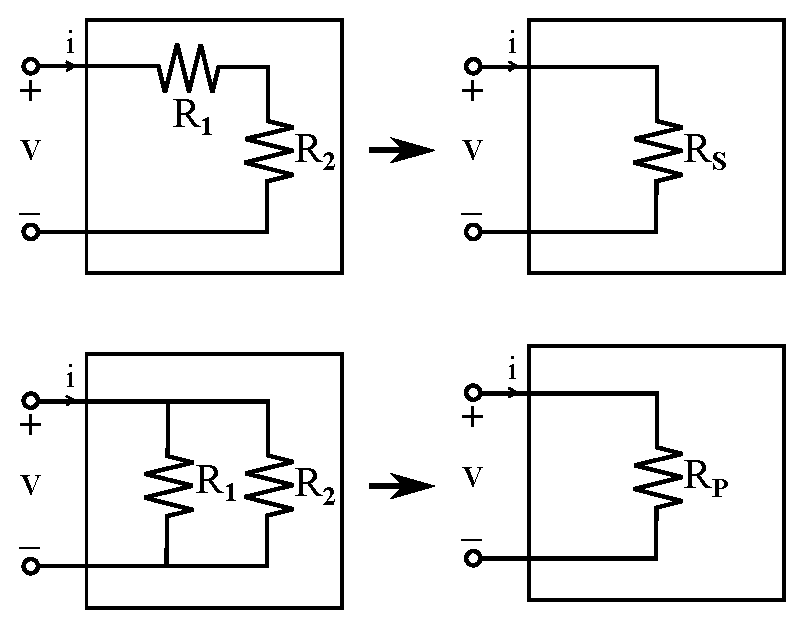
\includegraphics[width=1\textwidth,height=0.6\textheight]{./image/circuit1/appendix_end}
\end{figure}
\end{column}

\begin{column}{4cm}
\vspace{8 mm} \newline
$v = R_1I + R_2I$ \newline
$v = R_sI$ \newline
$\therefore R_s = R_1 + R_2$ \newline

\vspace{10 mm}
$R_p = \frac{1}{1/R_1+1/R_2} =\frac{R_1R_2}{R_1+R_2}$ \newline\newline
$ = R_1 \parallel R_2$

\end{column}

\begin{column}{2cm}
\bf{\orange{Series}} \newline\newline\newline\newline\newline

\bf{\orange{Parallel}}
\end{column}
\end{columns}

\end{frame}

%------------------------------------------------
%------------------------------------------------
\begin{frame}
\frametitle{Appendix(Voltage/Current Divider)}
\begin{columns}
\begin{column}{4.2cm}
\begin{figure}[H]
  \centering
  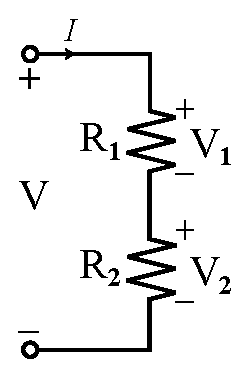
\includegraphics[width=0.5\textwidth,height=0.4\textheight]{./image/circuit1/append_end2}
\end{figure}
\begin{itemize} \itemsep1pt \parskip0pt \parsep0pt
	\item[] $I=\frac{V}{R_1 + R_2}$
	\item[] $V_1 = R_1I = \frac{R_1}{R_1 + R_2}V$
	\item[] $V_2 = R_2I = \frac{R_2}{R_1 + R_2}V$
\end{itemize}
\end{column}

\begin{column}{4cm}
$\leftarrow $ \bf{\orange{Voltage Divider}}
\vspace{16 mm} \newline
\bf{\orange{Current Divider}} $\rightarrow $
\end{column}

\begin{column}{4cm}
\begin{figure}[H]
  \centering
  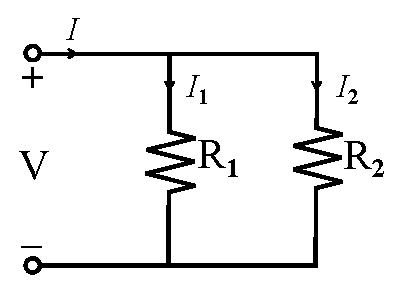
\includegraphics[width=0.8\textwidth,height=0.3\textheight]{./image/circuit1/append_end2_2}
\end{figure}
\begin{itemize} \itemsep1pt \parskip0pt \parsep0pt
	\item[] $V = (R_1 \parallel R_2)I$
	\item[] $I_1 = \frac{V}{R_1} = \frac{R_1\parallel R_2}{R_1}I = \frac{R_2}{R_1+R_2}I$
	\item[] $I_2 = \frac{R_1}{R_1 + R_2}I$
\end{itemize}
\end{column}
\end{columns}
\end{frame}

%------------------------------------------------




















% \begin{frame}
% \frametitle{Multiple Columns}
% \begin{columns}[c] % The "c" option specifies centered vertical alignment while the "t" option is used for top vertical alignment

% \column{.45\textwidth} % Left column and width
% \textbf{Heading}
% \begin{enumerate}
% \item Statement
% \item Explanation
% \item Example
% \end{enumerate}

% \column{.5\textwidth} % Right column and width
% Lorem ipsum dolor sit amet, consectetur adipiscing elit. Integer lectus nisl, ultricies in feugiat rutrum, porttitor sit amet augue. Aliquam ut tortor mauris. Sed volutpat ante purus, quis accumsan dolor.

% \end{columns}
% \end{frame}

% %------------------------------------------------
% \section{Second Section}
% %------------------------------------------------

% \begin{frame}
% \frametitle{Table}
% \begin{table}
% \begin{tabular}{l l l}
% \toprule
% \textbf{Treatments} & \textbf{Response 1} & \textbf{Response 2}\\
% \midrule
% Treatment 1 & 0.0003262 & 0.562 \\
% Treatment 2 & 0.0015681 & 0.910 \\
% Treatment 3 & 0.0009271 & 0.296 \\
% \bottomrule
% \end{tabular}
% \caption{Table caption}
% \end{table}
% \end{frame}

% %------------------------------------------------

% \begin{frame}
% \frametitle{Theorem}
% \begin{theorem}[Mass--energy equivalence]
% $E = mc^2$
% \end{theorem}
% \end{frame}

% %------------------------------------------------

% \begin{frame}[fragile] % Need to use the fragile option when verbatim is used in the slide
% \frametitle{Verbatim}
% \begin{example}[Theorem Slide Code]
% \begin{verbatim}
% \begin{frame}
% \frametitle{Theorem}
% \begin{theorem}[Mass--energy equivalence]
% $E = mc^2$
% \end{theorem}
% \end{frame}\end{verbatim}
% \end{example}
% \end{frame}

% %------------------------------------------------

% \begin{frame}
% \frametitle{Figure}
% Uncomment the code on this slide to include your own image from the same directory as the template .TeX file.
% %\begin{figure}
% %\includegraphics[width=0.8\linewidth]{test}
% %\end{figure}
% \end{frame}

% %------------------------------------------------

% \begin{frame}[fragile] % Need to use the fragile option when verbatim is used in the slide
% \frametitle{Citation}
% An example of the \verb|\cite| command to cite within the presentation:\\~

% This statement requires citation \cite{p1}.
% \end{frame}

% ------------------------------------------------

% \begin{frame}
% \frametitle{References}
% \footnotesize{
% \begin{thebibliography}{99} % Beamer does not support BibTeX so references must be inserted manually as below
% \bibitem[Smith, 2012]{p1} John Smith (2012)
% \newblock Title of the publication
% \newblock \emph{Journal Name} 12(3), 45 -- 678.
% \end{thebibliography}
% }
% \end{frame}

% %------------------------------------------------

\begin{frame}
\Huge{\centerline{The End}}
\end{frame}

%----------------------------------------------------------------------------------------

\end{document}